\documentclass[pdf, unicode, 12pt, a4paper,oneside,fleqn]{article}

\usepackage{styles/log-style}
\begin{document}

\begin{titlepage}
\begin{center}
\bfseries
{\Large Московский авиационный институт\\ (национальный исследовательский университет)}

\vspace{48pt}
{\large Факультет информационных технологий и прикладной математики}

\vspace{36pt}
{\large Кафедра вычислительной математики и программирования}

\vspace{48pt}Курсовой проект по курсу 
\enquote{Численные методы}
\end{center}
\vspace{72pt}

\begin{flushright}
\begin{tabular}{rl}
Студент: & П.\,А. Гамов \\
Преподаватель: & Д.\,Л. Ревизников \\
Группа: & М8О-407Б \\
Дата: & \\
Оценка: & \\
Подпись: & \\
\end{tabular}
\end{flushright}
\vfill
\begin{center}
\bfseries
Москва, \the\year
\end{center}
\end{titlepage}

\pagebreak

\CWHeader{Сингулярное разложение матриц}

\section{Введение}

Сингулярное разложение — определённого типа разложение прямоугольной матрицы. Имеющее широкое применение, в силу своей наглядной геометрической интерпретации, при решении многих прикладных задач. Переформулировка сингулярного разложения, так называемое разложение Шмидта имеет приложения в квантовой теории информации, например в запутанности.

Сингулярное разложение матрицы $M$ позволяет вычислять сингулярные числа данной матрицы, а также левые и правые сингулярные векторы матрицы $M$:

левые сингулярные векторы матрицы $M$ — это собственные векторы матрицы  $M^*M.$;

правые сингулярные векторы матрицы $M$ — это собственные векторы матрицы $M^*M.$

Сингулярное разложение является удобным при вычислении ранга матрицы, ядра матрицы и псевдообратной матрицы.

Сингулярное разложение также используется для приближения матриц матрицами заданного ранга.

\section{Определение}

Сингулярным разложением матрицы $M$ порядка  $m \times n$ является разложение следующего вида

$$
M = U \Sigma V^{*}
$$

где $\Sigma$  — матрица размера $m \times n$ с неотрицательными элементами, у которой элементы, лежащие на главной диагонали — это сингулярные числа (а все элементы, не лежащие на главной диагонали, являются нулевыми), а матрицы $U$ (порядка $m$) и $V$ (порядка $n$) — это две унитарные матрицы, состоящие из левых и правых сингулярных векторов соответственно (а $V^*$ — это сопряжённо-транспонированная матрица к $V$).

Пусть дана матрица:

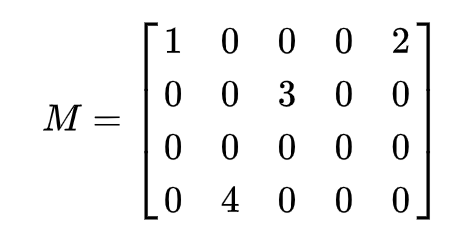
\includegraphics[scale=0.4]{data1.png}

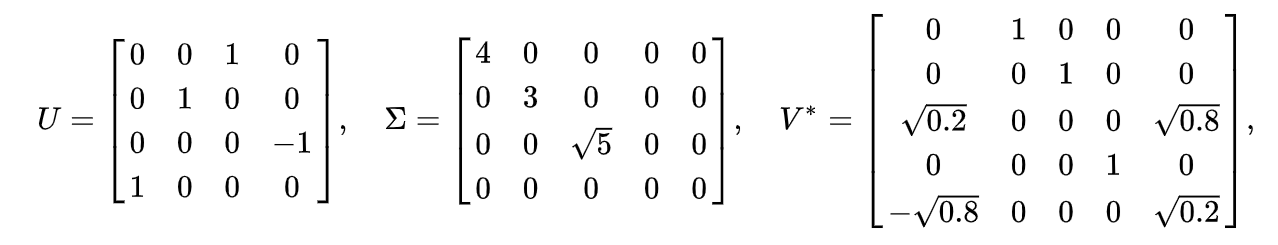
\includegraphics[scale=0.35]{data2.png}

\section{Вращения Якоби}

Для нахождения собственных чисел и сопряженных векторов используем алгоритм вращений Якоби.

\begin{lstlisting}
def jacobi(A):
    err = 0.1
    U = None
    while True:
        i, j = find_max(A)
        P = math.pi / 4
        if A[i][i] - A[j][j] != 0:
            P = 2 * A[i][j] / (A[i][i] - A[j][j])
        c = math.cos(math.atan(P) / 2)
        s = math.sin(math.atan(P) / 2)
        rotate = rotate_matrix(len(A),s,c,i,j)
        if U == None:
            U = copy.deepcopy(rotate)
        else:
            U = prois(U, rotate)
        A = prois(prois(transpose(rotate),A),rotate)
        er = error(A)
        if er < err:
            break
    res = []
    for i in range(len(A)):
        vec = [U[j][i] for j in range(len(A))]
        vecs = sum([x**2 for x in vec])**0.5
        if vecs != 0:
            vec = [x / vecs for x in vec]
        res.append([A[i][i],vec])
    return res
\end{lstlisting}

Цепочка произведений матриц поворота дает нам матрицу состоящую из собственных векторов.
Далее после нормировки они возвращаются из функции.

\section{SVD}

\begin{lstlisting}
def SVD(A, cut=0):
    A1res = sorted(jacobi(prois(transpose(A),A)))[::-1]
    right = [[A1res[i][1][j] for j in range(len(A1res))] for i in range(len(A1res))]
    A2res = sorted(jacobi(prois(A,transpose(A))))[::-1]
    left = [[A2res[j][1][i] for j in range(len(A2res))] for i in range(len(A2res))]
    center = [[0 for j in range(len(A[i]))] for i in range(len(A))]
    for i in range(min(len(A),len(A[0]))):
        center[i][i] = A1res[i][0]**0.5
    if cut != 0 and cut < 100:
        f_vert = max(math.floor(len(center) * (100 - cut) / 100),1)
        f_hor = max(math.floor(len(center[0]) * (100 - cut) / 100),1)
        left = [[left[i][j] for j in range(f_vert)] for i in range(len(left))]
        right = [[right[i][j] for j in range(len(right[0]))] for i in range(f_hor)]
        center = [[center[i][j] for j in range(f_hor)] for i in range(f_vert)]
        return left, center, right
    else:
        return left, center, right
\end{lstlisting}

Если нет второго параметра, то алгоритм вернет 3 матрицы разложения, если есть параметр cut, то алгоритм обрежет разложение и вернет обрезаные компоненты матриц, которые содержат самые большие сингулярные числа.

\begin{lstlisting}
A = [[1,0,0,0,2],
     [0,0,3,0,0],
     [0,0,0,0,0],
     [0,4,0,0,0]]
\end{lstlisting}

Рассмотрим на матрице из примера выше.

Левая компонента разложения.

\begin{lstlisting}
array([[ 0.,  0.,  1.,  0.],
       [ 0.,  1., -0.,  0.],
       [ 0.,  0.,  0.,  1.],
       [ 1.,  0.,  0.,  0.]])
\end{lstlisting}

Центральная компонента разложения. Содержит в себе синулярные числа в порядке убывания.

\begin{lstlisting}
array([[4.        , 0.        , 0.        , 0.        , 0.        ],
       [0.        , 3.        , 0.        , 0.        , 0.        ],
       [0.        , 0.        , 2.23606798, 0.        , 0.        ],
       [0.        , 0.        , 0.        , 0.        , 0.        ]])
\end{lstlisting}

Правая компонента разложения.

\begin{lstlisting}
array([[ 0.        ,  1.        ,  0.        ,  0.        ,  0.        ],
       [ 0.        ,  0.        ,  1.        ,  0.        ,  0.        ],
       [ 0.4472136 ,  0.        ,  0.        ,  0.        ,  0.89442719],
       [ 0.89442719,  0.        ,  0.        ,  0.        , -0.4472136 ],
       [ 0.        ,  0.        ,  0.        ,  1.        ,  0.        ]])
\end{lstlisting}

Если умножить матрицы по порядку мы получим исходную матрицу.

\begin{lstlisting}
[[1.0, 0.0, 0.0, 0.0, 2.0],
 [0.0, 0.0, 3.0, 0.0, 0.0],
 [0.0, 0.0, 0.0, 0.0, 0.0],
 [0.0, 4.0, 0.0, 0.0, 0.0]]
\end{lstlisting}

Теперь попробуем обрезать одно сингулярное число.

Левая компонента разложения.

\begin{lstlisting}
array([[0., 0.],
       [0., 1.],
       [0., 0.],
       [1., 0.]])
\end{lstlisting}

Центральная компонента разложения.

\begin{lstlisting}
array([[4., 0.],
       [0., 3.]])
\end{lstlisting}

Правая компонента разложения.

\begin{lstlisting}
array([[0., 1., 0., 0., 0.],
       [0., 0., 1., 0., 0.]])
\end{lstlisting}

Если умножить матрицы по порядку мы получим исходную матрицу.

\begin{lstlisting}
[[0.0, 0.0, 0.0, 0.0, 0.0],
 [0.0, 0.0, 3.0, 0.0, 0.0],
 [0.0, 0.0, 0.0, 0.0, 0.0],
 [0.0, 4.0, 0.0, 0.0, 0.0]]
\end{lstlisting}

Для такой маленькой матрицы первая строчка обратилась в ноль. Данные потеряны. На большей матрице с большим рангом потеря окажется несущественной.

Такое отрезание менее значимых компонент составляет основу применений данного разложения: используя данный алгоритм, можно получить наилучную апроксимацию матрицы рангом не больше некого заданного числа. А значит данный алгоритм можно использовать например для сжатия картинок без существенной потери качества.

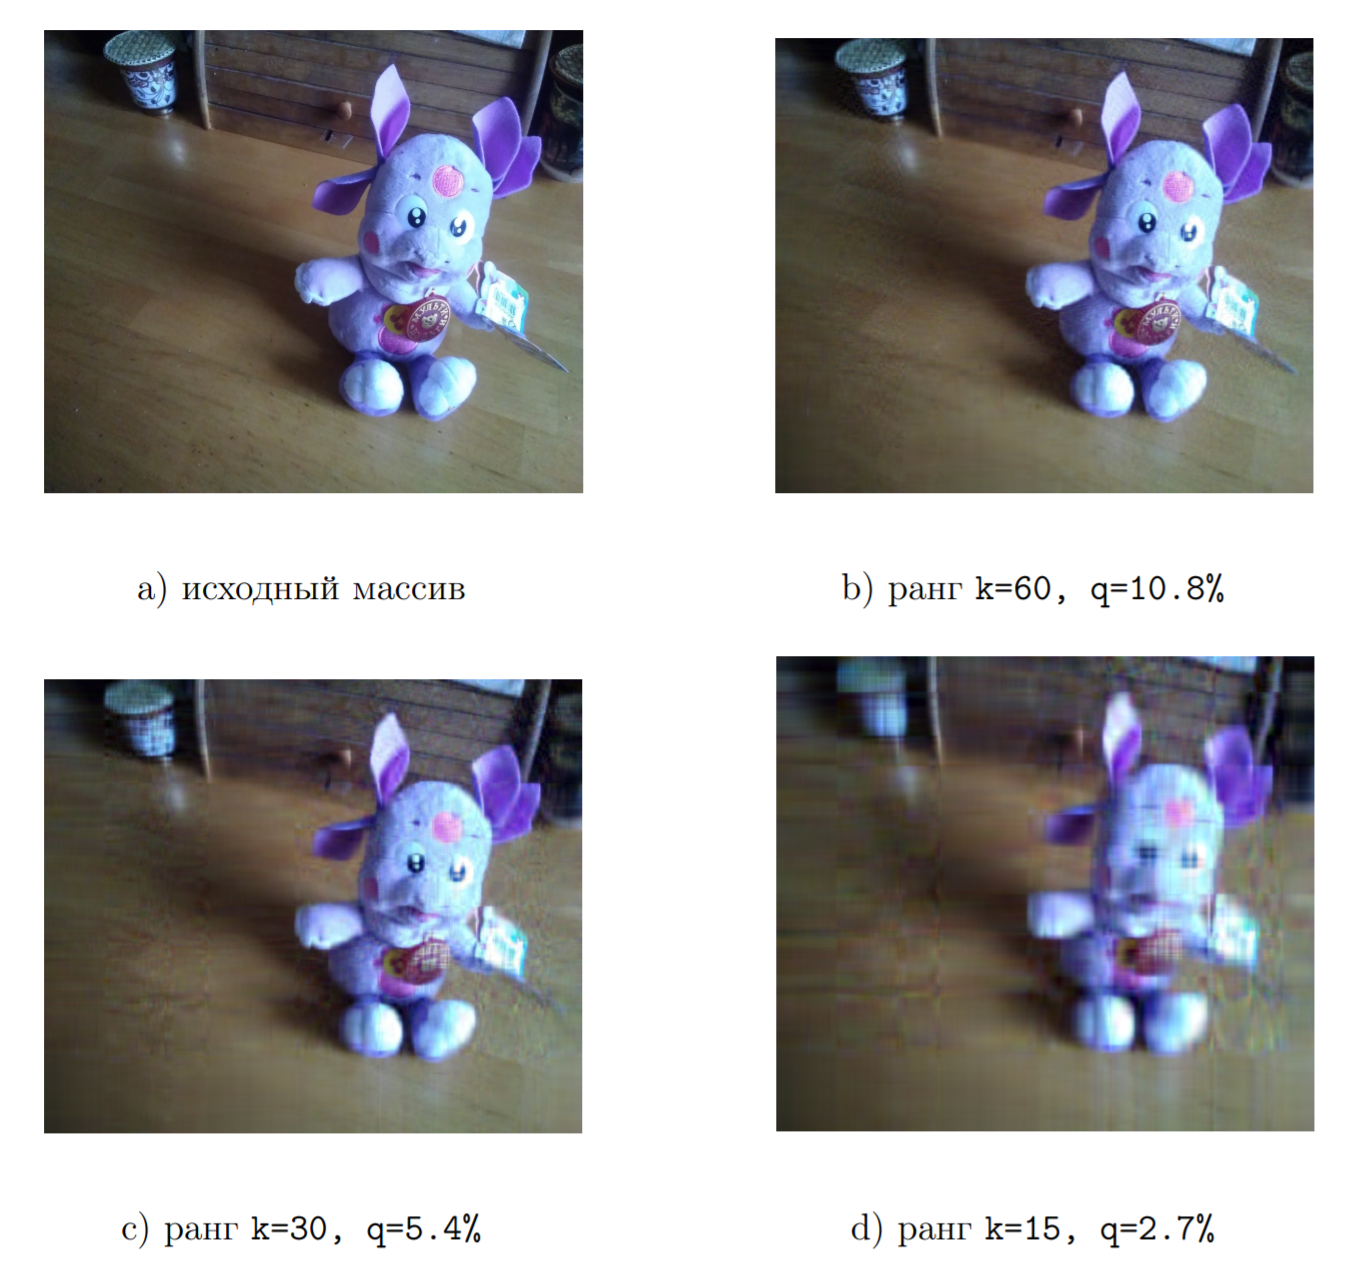
\includegraphics[scale=0.3]{data3.png}

Материал взят из работы Карчевского М.М.

\section{Выводы}

Сингулярное разложение позволяет понизить ранг матрицы, что имеет свое применение в математике. Так же разложение имеет прикладное применение, такое как сжатие изображений, апроксимация графиков и данных.

\end{document}